\documentclass[twoside]{book}

% Packages required by doxygen
\usepackage{fixltx2e}
\usepackage{calc}
\usepackage{doxygen}
\usepackage[export]{adjustbox} % also loads graphicx
\usepackage{graphicx}
\usepackage[utf8]{inputenc}
\usepackage{makeidx}
\usepackage{multicol}
\usepackage{multirow}
\PassOptionsToPackage{warn}{textcomp}
\usepackage{textcomp}
\usepackage[nointegrals]{wasysym}
\usepackage[table]{xcolor}

% Font selection
\usepackage[T1]{fontenc}
\usepackage[scaled=.90]{helvet}
\usepackage{courier}
\usepackage{amssymb}
\usepackage{sectsty}
\renewcommand{\familydefault}{\sfdefault}
\allsectionsfont{%
  \fontseries{bc}\selectfont%
  \color{darkgray}%
}
\renewcommand{\DoxyLabelFont}{%
  \fontseries{bc}\selectfont%
  \color{darkgray}%
}
\newcommand{\+}{\discretionary{\mbox{\scriptsize$\hookleftarrow$}}{}{}}

% Page & text layout
\usepackage{geometry}
\geometry{%
  a4paper,%
  top=2.5cm,%
  bottom=2.5cm,%
  left=2.5cm,%
  right=2.5cm%
}
\tolerance=750
\hfuzz=15pt
\hbadness=750
\setlength{\emergencystretch}{15pt}
\setlength{\parindent}{0cm}
\setlength{\parskip}{3ex plus 2ex minus 2ex}
\makeatletter
\renewcommand{\paragraph}{%
  \@startsection{paragraph}{4}{0ex}{-1.0ex}{1.0ex}{%
    \normalfont\normalsize\bfseries\SS@parafont%
  }%
}
\renewcommand{\subparagraph}{%
  \@startsection{subparagraph}{5}{0ex}{-1.0ex}{1.0ex}{%
    \normalfont\normalsize\bfseries\SS@subparafont%
  }%
}
\makeatother

% Headers & footers
\usepackage{fancyhdr}
\pagestyle{fancyplain}
\fancyhead[LE]{\fancyplain{}{\bfseries\thepage}}
\fancyhead[CE]{\fancyplain{}{}}
\fancyhead[RE]{\fancyplain{}{\bfseries\leftmark}}
\fancyhead[LO]{\fancyplain{}{\bfseries\rightmark}}
\fancyhead[CO]{\fancyplain{}{}}
\fancyhead[RO]{\fancyplain{}{\bfseries\thepage}}
\fancyfoot[LE]{\fancyplain{}{}}
\fancyfoot[CE]{\fancyplain{}{}}
\fancyfoot[RE]{\fancyplain{}{\bfseries\scriptsize Generated by Doxygen }}
\fancyfoot[LO]{\fancyplain{}{\bfseries\scriptsize Generated by Doxygen }}
\fancyfoot[CO]{\fancyplain{}{}}
\fancyfoot[RO]{\fancyplain{}{}}
\renewcommand{\footrulewidth}{0.4pt}
\renewcommand{\chaptermark}[1]{%
  \markboth{#1}{}%
}
\renewcommand{\sectionmark}[1]{%
  \markright{\thesection\ #1}%
}

% Indices & bibliography
\usepackage{natbib}
\usepackage[titles]{tocloft}
\setcounter{tocdepth}{3}
\setcounter{secnumdepth}{5}
\makeindex

% Hyperlinks (required, but should be loaded last)
\usepackage{ifpdf}
\ifpdf
  \usepackage[pdftex,pagebackref=true]{hyperref}
\else
  \usepackage[ps2pdf,pagebackref=true]{hyperref}
\fi
\hypersetup{%
  colorlinks=true,%
  linkcolor=blue,%
  citecolor=blue,%
  unicode%
}

% Custom commands
\newcommand{\clearemptydoublepage}{%
  \newpage{\pagestyle{empty}\cleardoublepage}%
}

\usepackage{caption}
\captionsetup{labelsep=space,justification=centering,font={bf},singlelinecheck=off,skip=4pt,position=top}

%===== C O N T E N T S =====

\begin{document}

% Titlepage & ToC
\hypersetup{pageanchor=false,
             bookmarksnumbered=true,
             pdfencoding=unicode
            }
\pagenumbering{alph}
\begin{titlepage}
\vspace*{7cm}
\begin{center}%
{\Large 07-\/cmd }\\
\vspace*{1cm}
{\large Generated by Doxygen 1.8.13}\\
\end{center}
\end{titlepage}
\clearemptydoublepage
\pagenumbering{roman}
\tableofcontents
\clearemptydoublepage
\pagenumbering{arabic}
\hypersetup{pageanchor=true}

%--- Begin generated contents ---
\chapter{Namespace Index}
\section{Namespace List}
Here is a list of all namespaces with brief descriptions\+:\begin{DoxyCompactList}
\item\contentsline{section}{\hyperlink{namespacematrix}{matrix} }{\pageref{namespacematrix}}{}
\item\contentsline{section}{\hyperlink{namespacematrix_1_1detail}{matrix\+::detail} }{\pageref{namespacematrix_1_1detail}}{}
\end{DoxyCompactList}

\chapter{Hierarchical Index}
\section{Class Hierarchy}
This inheritance list is sorted roughly, but not completely, alphabetically\+:\begin{DoxyCompactList}
\item \contentsline{section}{bayan\+:\+:hash\+:\+:hash}{\pageref{classbayan_1_1hash_1_1hash}}{}
\begin{DoxyCompactList}
\item \contentsline{section}{bayan\+:\+:hash\+:\+:md5}{\pageref{classbayan_1_1hash_1_1md5}}{}
\end{DoxyCompactList}
\item \contentsline{section}{bayan\+:\+:options}{\pageref{structbayan_1_1options}}{}
\end{DoxyCompactList}

\chapter{Class Index}
\section{Class List}
Here are the classes, structs, unions and interfaces with brief descriptions\+:\begin{DoxyCompactList}
\item\contentsline{section}{\hyperlink{classedu__allocator}{edu\+\_\+allocator$<$ T, batch\+\_\+count $>$} }{\pageref{classedu__allocator}}{}
\item\contentsline{section}{\hyperlink{classedu__container}{edu\+\_\+container$<$ T, size, Alloc $>$} }{\pageref{classedu__container}}{}
\item\contentsline{section}{\hyperlink{structedu__allocator_1_1rebind}{edu\+\_\+allocator$<$ T, batch\+\_\+count $>$\+::rebind$<$ U $>$} }{\pageref{structedu__allocator_1_1rebind}}{}
\end{DoxyCompactList}

\chapter{File Index}
\section{File List}
Here is a list of all files with brief descriptions\+:\begin{DoxyCompactList}
\item\contentsline{section}{src/\hyperlink{block__printer_8cpp}{block\+\_\+printer.\+cpp} }{\pageref{block__printer_8cpp}}{}
\item\contentsline{section}{src/\hyperlink{block__printer_8hpp}{block\+\_\+printer.\+hpp} }{\pageref{block__printer_8hpp}}{}
\item\contentsline{section}{src/\hyperlink{block__reader_8cpp}{block\+\_\+reader.\+cpp} }{\pageref{block__reader_8cpp}}{}
\item\contentsline{section}{src/\hyperlink{block__reader_8hpp}{block\+\_\+reader.\+hpp} }{\pageref{block__reader_8hpp}}{}
\item\contentsline{section}{src/\hyperlink{line__reader_8cpp}{line\+\_\+reader.\+cpp} }{\pageref{line__reader_8cpp}}{}
\item\contentsline{section}{src/\hyperlink{line__reader_8hpp}{line\+\_\+reader.\+hpp} }{\pageref{line__reader_8hpp}}{}
\item\contentsline{section}{src/\hyperlink{main_8cpp}{main.\+cpp} }{\pageref{main_8cpp}}{}
\item\contentsline{section}{src/\hyperlink{observable_8hpp}{observable.\+hpp} }{\pageref{observable_8hpp}}{}
\end{DoxyCompactList}

\chapter{Namespace Documentation}
\hypertarget{namespacebulk}{}\section{bulk Namespace Reference}
\label{namespacebulk}\index{bulk@{bulk}}
\subsection*{Classes}
\begin{DoxyCompactItemize}
\item 
class \hyperlink{classbulk_1_1AbstractObservable}{Abstract\+Observable}
\item 
class \hyperlink{classbulk_1_1BlockPrinter}{Block\+Printer}
\item 
class \hyperlink{classbulk_1_1BlockReader}{Block\+Reader}
\item 
class \hyperlink{classbulk_1_1LineReader}{Line\+Reader}
\item 
class \hyperlink{classbulk_1_1Observable}{Observable}
\item 
class \hyperlink{classbulk_1_1Observer}{Observer}
\end{DoxyCompactItemize}

\chapter{Class Documentation}
\hypertarget{classbulk_1_1AbstractObservable}{}\section{bulk\+:\+:Abstract\+Observable$<$ T $>$ Class Template Reference}
\label{classbulk_1_1AbstractObservable}\index{bulk\+::\+Abstract\+Observable$<$ T $>$@{bulk\+::\+Abstract\+Observable$<$ T $>$}}


{\ttfamily \#include $<$observable.\+hpp$>$}

Inheritance diagram for bulk\+:\+:Abstract\+Observable$<$ T $>$\+:\begin{figure}[H]
\begin{center}
\leavevmode
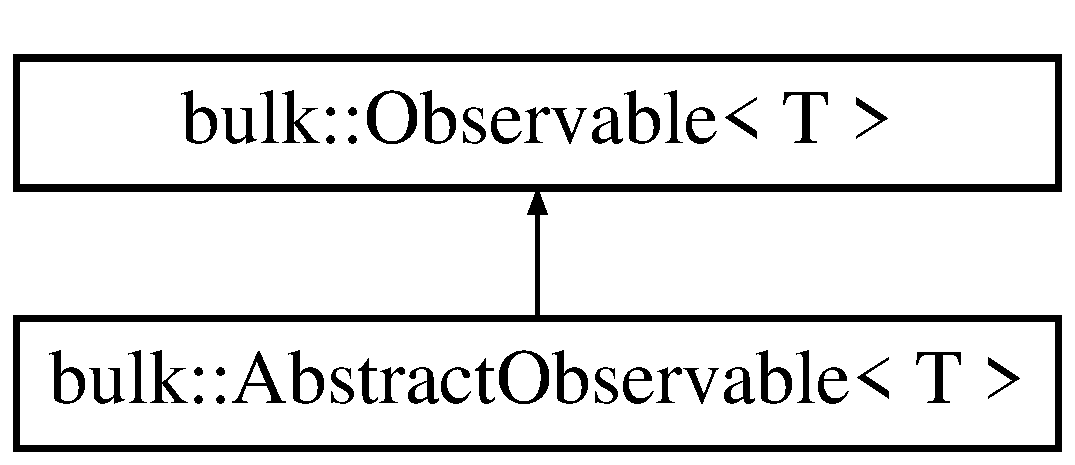
\includegraphics[height=2.000000cm]{classbulk_1_1AbstractObservable}
\end{center}
\end{figure}
\subsection*{Public Member Functions}
\begin{DoxyCompactItemize}
\item 
\hyperlink{classbulk_1_1AbstractObservable_a8fe881a61345c8df0c201a2e266605ef}{$\sim$\+Abstract\+Observable} () override=default
\item 
void \hyperlink{classbulk_1_1AbstractObservable_a39be332eeed3b432a461faae184ba34b}{add\+\_\+subscriber} (const std\+::shared\+\_\+ptr$<$ \hyperlink{classbulk_1_1Observer}{Observer}$<$ T $>$$>$ \&observer) override
\end{DoxyCompactItemize}
\subsection*{Protected Member Functions}
\begin{DoxyCompactItemize}
\item 
void \hyperlink{classbulk_1_1AbstractObservable_a95ccf77b0c8774129fd1d2b25642356e}{emit} (const T \&data)
\end{DoxyCompactItemize}


\subsection{Detailed Description}
\subsubsection*{template$<$typename T$>$\newline
class bulk\+::\+Abstract\+Observable$<$ T $>$}

Abstract implementation of \hyperlink{classbulk_1_1Observable}{Observable} that stores forward\+\_\+list of weak pointers to Observers 
\begin{DoxyTemplParams}{Template Parameters}
{\em T} & \hyperlink{classbulk_1_1Observable}{Observable} data type \\
\hline
\end{DoxyTemplParams}


\subsection{Constructor \& Destructor Documentation}
\mbox{\Hypertarget{classbulk_1_1AbstractObservable_a8fe881a61345c8df0c201a2e266605ef}\label{classbulk_1_1AbstractObservable_a8fe881a61345c8df0c201a2e266605ef}} 
\index{bulk\+::\+Abstract\+Observable@{bulk\+::\+Abstract\+Observable}!````~Abstract\+Observable@{$\sim$\+Abstract\+Observable}}
\index{````~Abstract\+Observable@{$\sim$\+Abstract\+Observable}!bulk\+::\+Abstract\+Observable@{bulk\+::\+Abstract\+Observable}}
\subsubsection{\texorpdfstring{$\sim$\+Abstract\+Observable()}{~AbstractObservable()}}
{\footnotesize\ttfamily template$<$typename T$>$ \\
\hyperlink{classbulk_1_1AbstractObservable}{bulk\+::\+Abstract\+Observable}$<$ T $>$\+::$\sim$\hyperlink{classbulk_1_1AbstractObservable}{Abstract\+Observable} (\begin{DoxyParamCaption}{ }\end{DoxyParamCaption})\hspace{0.3cm}{\ttfamily [override]}, {\ttfamily [default]}}



\subsection{Member Function Documentation}
\mbox{\Hypertarget{classbulk_1_1AbstractObservable_a39be332eeed3b432a461faae184ba34b}\label{classbulk_1_1AbstractObservable_a39be332eeed3b432a461faae184ba34b}} 
\index{bulk\+::\+Abstract\+Observable@{bulk\+::\+Abstract\+Observable}!add\+\_\+subscriber@{add\+\_\+subscriber}}
\index{add\+\_\+subscriber@{add\+\_\+subscriber}!bulk\+::\+Abstract\+Observable@{bulk\+::\+Abstract\+Observable}}
\subsubsection{\texorpdfstring{add\+\_\+subscriber()}{add\_subscriber()}}
{\footnotesize\ttfamily template$<$typename T$>$ \\
void \hyperlink{classbulk_1_1AbstractObservable}{bulk\+::\+Abstract\+Observable}$<$ T $>$\+::add\+\_\+subscriber (\begin{DoxyParamCaption}\item[{const std\+::shared\+\_\+ptr$<$ \hyperlink{classbulk_1_1Observer}{Observer}$<$ T $>$$>$ \&}]{observer }\end{DoxyParamCaption})\hspace{0.3cm}{\ttfamily [inline]}, {\ttfamily [override]}, {\ttfamily [virtual]}}

Adds a subscriber (observer) to the list 
\begin{DoxyParams}{Parameters}
{\em observer} & \hyperlink{classbulk_1_1Observer}{Observer} to be added \\
\hline
\end{DoxyParams}


Implements \hyperlink{classbulk_1_1Observable_a1d014ef91398bff19bf96d9ef6bd5e10}{bulk\+::\+Observable$<$ T $>$}.

\mbox{\Hypertarget{classbulk_1_1AbstractObservable_a95ccf77b0c8774129fd1d2b25642356e}\label{classbulk_1_1AbstractObservable_a95ccf77b0c8774129fd1d2b25642356e}} 
\index{bulk\+::\+Abstract\+Observable@{bulk\+::\+Abstract\+Observable}!emit@{emit}}
\index{emit@{emit}!bulk\+::\+Abstract\+Observable@{bulk\+::\+Abstract\+Observable}}
\subsubsection{\texorpdfstring{emit()}{emit()}}
{\footnotesize\ttfamily template$<$typename T$>$ \\
void \hyperlink{classbulk_1_1AbstractObservable}{bulk\+::\+Abstract\+Observable}$<$ T $>$\+::emit (\begin{DoxyParamCaption}\item[{const T \&}]{data }\end{DoxyParamCaption})\hspace{0.3cm}{\ttfamily [inline]}, {\ttfamily [protected]}}

Emit data, notifying each observer 
\begin{DoxyParams}{Parameters}
{\em data} & Data to be emitted \\
\hline
\end{DoxyParams}


The documentation for this class was generated from the following file\+:\begin{DoxyCompactItemize}
\item 
src/\hyperlink{observable_8hpp}{observable.\+hpp}\end{DoxyCompactItemize}

\hypertarget{classbulk_1_1BlockFilePrinter}{}\section{bulk\+:\+:Block\+File\+Printer Class Reference}
\label{classbulk_1_1BlockFilePrinter}\index{bulk\+::\+Block\+File\+Printer@{bulk\+::\+Block\+File\+Printer}}


Saves each block into a separate file file name format\+: bulk123456.\+log Where 123456 is the timestamp in seconds.  




{\ttfamily \#include $<$block\+\_\+file\+\_\+printer.\+hpp$>$}

Inheritance diagram for bulk\+:\+:Block\+File\+Printer\+:\begin{figure}[H]
\begin{center}
\leavevmode
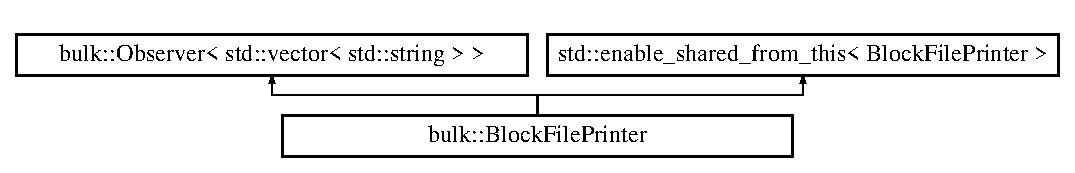
\includegraphics[height=1.879195cm]{classbulk_1_1BlockFilePrinter}
\end{center}
\end{figure}
\subsection*{Public Member Functions}
\begin{DoxyCompactItemize}
\item 
\hyperlink{classbulk_1_1BlockFilePrinter_af93de98e11a9c3881ab6bbc7ab90de61}{$\sim$\+Block\+File\+Printer} () override=default
\item 
void \hyperlink{classbulk_1_1BlockFilePrinter_a3e8a6eaf52ef8bef0fa9ec0b298c7382}{update} (const std\+::vector$<$ std\+::string $>$ \&data) override
\end{DoxyCompactItemize}
\subsection*{Static Public Member Functions}
\begin{DoxyCompactItemize}
\item 
static std\+::shared\+\_\+ptr$<$ \hyperlink{classbulk_1_1BlockFilePrinter}{Block\+File\+Printer} $>$ \hyperlink{classbulk_1_1BlockFilePrinter_a595744d305a5ffedce26f5a1a764142b}{create} ()
\end{DoxyCompactItemize}


\subsection{Detailed Description}
Saves each block into a separate file file name format\+: bulk123456.\+log Where 123456 is the timestamp in seconds. 

\subsection{Constructor \& Destructor Documentation}
\mbox{\Hypertarget{classbulk_1_1BlockFilePrinter_af93de98e11a9c3881ab6bbc7ab90de61}\label{classbulk_1_1BlockFilePrinter_af93de98e11a9c3881ab6bbc7ab90de61}} 
\index{bulk\+::\+Block\+File\+Printer@{bulk\+::\+Block\+File\+Printer}!````~Block\+File\+Printer@{$\sim$\+Block\+File\+Printer}}
\index{````~Block\+File\+Printer@{$\sim$\+Block\+File\+Printer}!bulk\+::\+Block\+File\+Printer@{bulk\+::\+Block\+File\+Printer}}
\subsubsection{\texorpdfstring{$\sim$\+Block\+File\+Printer()}{~BlockFilePrinter()}}
{\footnotesize\ttfamily bulk\+::\+Block\+File\+Printer\+::$\sim$\+Block\+File\+Printer (\begin{DoxyParamCaption}{ }\end{DoxyParamCaption})\hspace{0.3cm}{\ttfamily [override]}, {\ttfamily [default]}}



\subsection{Member Function Documentation}
\mbox{\Hypertarget{classbulk_1_1BlockFilePrinter_a595744d305a5ffedce26f5a1a764142b}\label{classbulk_1_1BlockFilePrinter_a595744d305a5ffedce26f5a1a764142b}} 
\index{bulk\+::\+Block\+File\+Printer@{bulk\+::\+Block\+File\+Printer}!create@{create}}
\index{create@{create}!bulk\+::\+Block\+File\+Printer@{bulk\+::\+Block\+File\+Printer}}
\subsubsection{\texorpdfstring{create()}{create()}}
{\footnotesize\ttfamily std\+::shared\+\_\+ptr$<$ \hyperlink{classbulk_1_1BlockFilePrinter}{bulk\+::\+Block\+File\+Printer} $>$ bulk\+::\+Block\+File\+Printer\+::create (\begin{DoxyParamCaption}{ }\end{DoxyParamCaption})\hspace{0.3cm}{\ttfamily [static]}}

\mbox{\Hypertarget{classbulk_1_1BlockFilePrinter_a3e8a6eaf52ef8bef0fa9ec0b298c7382}\label{classbulk_1_1BlockFilePrinter_a3e8a6eaf52ef8bef0fa9ec0b298c7382}} 
\index{bulk\+::\+Block\+File\+Printer@{bulk\+::\+Block\+File\+Printer}!update@{update}}
\index{update@{update}!bulk\+::\+Block\+File\+Printer@{bulk\+::\+Block\+File\+Printer}}
\subsubsection{\texorpdfstring{update()}{update()}}
{\footnotesize\ttfamily void bulk\+::\+Block\+File\+Printer\+::update (\begin{DoxyParamCaption}\item[{const std\+::vector$<$ std\+::string $>$ \&}]{data }\end{DoxyParamCaption})\hspace{0.3cm}{\ttfamily [override]}, {\ttfamily [virtual]}}



Implements \hyperlink{classbulk_1_1Observer_af17104660bf8b287e467213c4efbee2e}{bulk\+::\+Observer$<$ std\+::vector$<$ std\+::string $>$ $>$}.



The documentation for this class was generated from the following files\+:\begin{DoxyCompactItemize}
\item 
src/\hyperlink{block__file__printer_8hpp}{block\+\_\+file\+\_\+printer.\+hpp}\item 
src/\hyperlink{block__file__printer_8cpp}{block\+\_\+file\+\_\+printer.\+cpp}\end{DoxyCompactItemize}

\hypertarget{classbulk_1_1BlockPrinter}{}\section{bulk\+:\+:Block\+Printer Class Reference}
\label{classbulk_1_1BlockPrinter}\index{bulk\+::\+Block\+Printer@{bulk\+::\+Block\+Printer}}


{\ttfamily \#include $<$block\+\_\+printer.\+hpp$>$}

Inheritance diagram for bulk\+:\+:Block\+Printer\+:\begin{figure}[H]
\begin{center}
\leavevmode
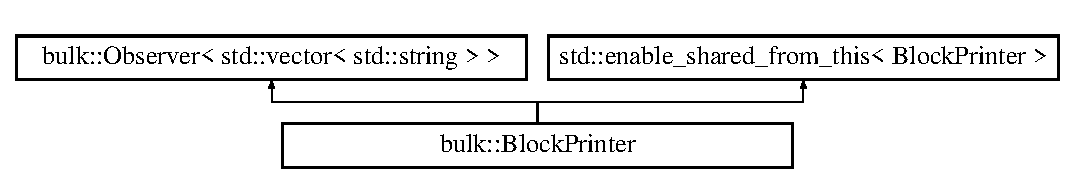
\includegraphics[height=2.000000cm]{classbulk_1_1BlockPrinter}
\end{center}
\end{figure}
\subsection*{Public Member Functions}
\begin{DoxyCompactItemize}
\item 
\hyperlink{classbulk_1_1BlockPrinter_ade61ac6f7602a0ee469244c98f43bc03}{$\sim$\+Block\+Printer} () override=default
\item 
void \hyperlink{classbulk_1_1BlockPrinter_a9f961b39d2c0bf9112524bf6773bb3e1}{update} (const std\+::vector$<$ std\+::string $>$ \&data) override
\end{DoxyCompactItemize}
\subsection*{Static Public Member Functions}
\begin{DoxyCompactItemize}
\item 
static std\+::shared\+\_\+ptr$<$ \hyperlink{classbulk_1_1BlockPrinter}{bulk\+::\+Block\+Printer} $>$ \hyperlink{classbulk_1_1BlockPrinter_ad0e918167006db76007fb2520ef3d228}{create} (std\+::ostream \&stream)
\end{DoxyCompactItemize}


\subsection{Detailed Description}
Prints incoming blocks (vectors of string) in format\+: \char`\"{}bulk\+: A, B, C$<$newline$>$\char`\"{} 

\subsection{Constructor \& Destructor Documentation}
\mbox{\Hypertarget{classbulk_1_1BlockPrinter_ade61ac6f7602a0ee469244c98f43bc03}\label{classbulk_1_1BlockPrinter_ade61ac6f7602a0ee469244c98f43bc03}} 
\index{bulk\+::\+Block\+Printer@{bulk\+::\+Block\+Printer}!````~Block\+Printer@{$\sim$\+Block\+Printer}}
\index{````~Block\+Printer@{$\sim$\+Block\+Printer}!bulk\+::\+Block\+Printer@{bulk\+::\+Block\+Printer}}
\subsubsection{\texorpdfstring{$\sim$\+Block\+Printer()}{~BlockPrinter()}}
{\footnotesize\ttfamily bulk\+::\+Block\+Printer\+::$\sim$\+Block\+Printer (\begin{DoxyParamCaption}{ }\end{DoxyParamCaption})\hspace{0.3cm}{\ttfamily [override]}, {\ttfamily [default]}}



\subsection{Member Function Documentation}
\mbox{\Hypertarget{classbulk_1_1BlockPrinter_ad0e918167006db76007fb2520ef3d228}\label{classbulk_1_1BlockPrinter_ad0e918167006db76007fb2520ef3d228}} 
\index{bulk\+::\+Block\+Printer@{bulk\+::\+Block\+Printer}!create@{create}}
\index{create@{create}!bulk\+::\+Block\+Printer@{bulk\+::\+Block\+Printer}}
\subsubsection{\texorpdfstring{create()}{create()}}
{\footnotesize\ttfamily std\+::shared\+\_\+ptr$<$ \hyperlink{classbulk_1_1BlockPrinter}{bulk\+::\+Block\+Printer} $>$ bulk\+::\+Block\+Printer\+::create (\begin{DoxyParamCaption}\item[{std\+::ostream \&}]{stream }\end{DoxyParamCaption})\hspace{0.3cm}{\ttfamily [static]}}

Create an instance of \hyperlink{classbulk_1_1BlockPrinter}{Block\+Printer} 
\begin{DoxyParams}{Parameters}
{\em stream} & Stream to write to \\
\hline
\end{DoxyParams}
\begin{DoxyReturn}{Returns}
Instance of \hyperlink{classbulk_1_1BlockPrinter}{Block\+Printer} 
\end{DoxyReturn}
\mbox{\Hypertarget{classbulk_1_1BlockPrinter_a9f961b39d2c0bf9112524bf6773bb3e1}\label{classbulk_1_1BlockPrinter_a9f961b39d2c0bf9112524bf6773bb3e1}} 
\index{bulk\+::\+Block\+Printer@{bulk\+::\+Block\+Printer}!update@{update}}
\index{update@{update}!bulk\+::\+Block\+Printer@{bulk\+::\+Block\+Printer}}
\subsubsection{\texorpdfstring{update()}{update()}}
{\footnotesize\ttfamily void bulk\+::\+Block\+Printer\+::update (\begin{DoxyParamCaption}\item[{const std\+::vector$<$ std\+::string $>$ \&}]{data }\end{DoxyParamCaption})\hspace{0.3cm}{\ttfamily [override]}, {\ttfamily [virtual]}}

Process (print) a block, function from \hyperlink{classbulk_1_1Observer}{Observer} 
\begin{DoxyParams}{Parameters}
{\em data} & \\
\hline
\end{DoxyParams}


Implements \hyperlink{classbulk_1_1Observer_af17104660bf8b287e467213c4efbee2e}{bulk\+::\+Observer$<$ std\+::vector$<$ std\+::string $>$ $>$}.



The documentation for this class was generated from the following files\+:\begin{DoxyCompactItemize}
\item 
src/\hyperlink{block__printer_8hpp}{block\+\_\+printer.\+hpp}\item 
src/\hyperlink{block__printer_8cpp}{block\+\_\+printer.\+cpp}\end{DoxyCompactItemize}

\hypertarget{classbulk_1_1BlockReader}{}\section{bulk\+:\+:Block\+Reader Class Reference}
\label{classbulk_1_1BlockReader}\index{bulk\+::\+Block\+Reader@{bulk\+::\+Block\+Reader}}


{\ttfamily \#include $<$block\+\_\+reader.\+hpp$>$}

Inheritance diagram for bulk\+:\+:Block\+Reader\+:\begin{figure}[H]
\begin{center}
\leavevmode
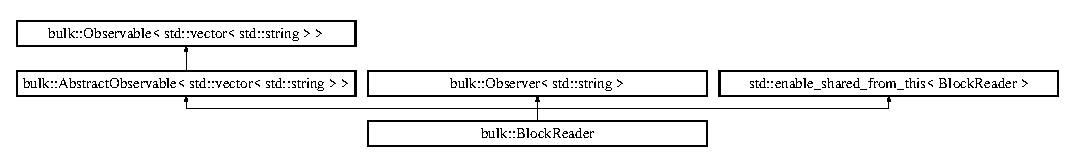
\includegraphics[height=1.744548cm]{classbulk_1_1BlockReader}
\end{center}
\end{figure}
\subsection*{Public Member Functions}
\begin{DoxyCompactItemize}
\item 
\hyperlink{classbulk_1_1BlockReader_a163856bf35ee489d5b2d0cae520fe89e}{$\sim$\+Block\+Reader} () override=default
\item 
void \hyperlink{classbulk_1_1BlockReader_a0a3b9ff69552b233b037afcd7e858ef1}{update} (const std\+::string \&data) override
\item 
void \hyperlink{classbulk_1_1BlockReader_a03c580cc41ffd5e3d1271eddba9ca261}{flush} ()
\end{DoxyCompactItemize}
\subsection*{Static Public Member Functions}
\begin{DoxyCompactItemize}
\item 
static std\+::shared\+\_\+ptr$<$ \hyperlink{classbulk_1_1BlockReader}{Block\+Reader} $>$ \hyperlink{classbulk_1_1BlockReader_af0d865e52b8882bf3ad7e2ee7de4c82e}{create} (size\+\_\+t \hyperlink{classbulk_1_1BlockReader_a368298f7d12180b3a59597b605154b1d}{block\+\_\+size})
\end{DoxyCompactItemize}
\subsection*{Public Attributes}
\begin{DoxyCompactItemize}
\item 
const size\+\_\+t \hyperlink{classbulk_1_1BlockReader_a368298f7d12180b3a59597b605154b1d}{block\+\_\+size}
\end{DoxyCompactItemize}
\subsection*{Additional Inherited Members}


\subsection{Detailed Description}
Reads blocks from stream of lines, emits blocks when they are formed correctly By default, a block is a vector of size determined by block\+\_\+size, but this can be changed if block contains commands like \{ and \} 

\subsection{Constructor \& Destructor Documentation}
\mbox{\Hypertarget{classbulk_1_1BlockReader_a163856bf35ee489d5b2d0cae520fe89e}\label{classbulk_1_1BlockReader_a163856bf35ee489d5b2d0cae520fe89e}} 
\index{bulk\+::\+Block\+Reader@{bulk\+::\+Block\+Reader}!````~Block\+Reader@{$\sim$\+Block\+Reader}}
\index{````~Block\+Reader@{$\sim$\+Block\+Reader}!bulk\+::\+Block\+Reader@{bulk\+::\+Block\+Reader}}
\subsubsection{\texorpdfstring{$\sim$\+Block\+Reader()}{~BlockReader()}}
{\footnotesize\ttfamily bulk\+::\+Block\+Reader\+::$\sim$\+Block\+Reader (\begin{DoxyParamCaption}{ }\end{DoxyParamCaption})\hspace{0.3cm}{\ttfamily [override]}, {\ttfamily [default]}}



\subsection{Member Function Documentation}
\mbox{\Hypertarget{classbulk_1_1BlockReader_af0d865e52b8882bf3ad7e2ee7de4c82e}\label{classbulk_1_1BlockReader_af0d865e52b8882bf3ad7e2ee7de4c82e}} 
\index{bulk\+::\+Block\+Reader@{bulk\+::\+Block\+Reader}!create@{create}}
\index{create@{create}!bulk\+::\+Block\+Reader@{bulk\+::\+Block\+Reader}}
\subsubsection{\texorpdfstring{create()}{create()}}
{\footnotesize\ttfamily std\+::shared\+\_\+ptr$<$ \hyperlink{classbulk_1_1BlockReader}{bulk\+::\+Block\+Reader} $>$ bulk\+::\+Block\+Reader\+::create (\begin{DoxyParamCaption}\item[{size\+\_\+t}]{block\+\_\+size }\end{DoxyParamCaption})\hspace{0.3cm}{\ttfamily [static]}}

Creates an instance of \hyperlink{classbulk_1_1BlockReader}{Block\+Reader} 
\begin{DoxyParams}{Parameters}
{\em block\+\_\+size} & Amount of lines the block will contain if input doesn\textquotesingle{}t have \{ or \} commands \\
\hline
\end{DoxyParams}
\begin{DoxyReturn}{Returns}
Instance of \hyperlink{classbulk_1_1BlockReader}{Block\+Reader} 
\end{DoxyReturn}
\mbox{\Hypertarget{classbulk_1_1BlockReader_a03c580cc41ffd5e3d1271eddba9ca261}\label{classbulk_1_1BlockReader_a03c580cc41ffd5e3d1271eddba9ca261}} 
\index{bulk\+::\+Block\+Reader@{bulk\+::\+Block\+Reader}!flush@{flush}}
\index{flush@{flush}!bulk\+::\+Block\+Reader@{bulk\+::\+Block\+Reader}}
\subsubsection{\texorpdfstring{flush()}{flush()}}
{\footnotesize\ttfamily void bulk\+::\+Block\+Reader\+::flush (\begin{DoxyParamCaption}{ }\end{DoxyParamCaption})}

Flushes (emits) a block, only if \char`\"{}\{\char`\"{} command wasn\textquotesingle{}t issued, or had \char`\"{}\}\char`\"{} that was paired to it \mbox{\Hypertarget{classbulk_1_1BlockReader_a0a3b9ff69552b233b037afcd7e858ef1}\label{classbulk_1_1BlockReader_a0a3b9ff69552b233b037afcd7e858ef1}} 
\index{bulk\+::\+Block\+Reader@{bulk\+::\+Block\+Reader}!update@{update}}
\index{update@{update}!bulk\+::\+Block\+Reader@{bulk\+::\+Block\+Reader}}
\subsubsection{\texorpdfstring{update()}{update()}}
{\footnotesize\ttfamily void bulk\+::\+Block\+Reader\+::update (\begin{DoxyParamCaption}\item[{const std\+::string \&}]{data }\end{DoxyParamCaption})\hspace{0.3cm}{\ttfamily [override]}, {\ttfamily [virtual]}}

Process a line 
\begin{DoxyParams}{Parameters}
{\em data} & Line without trailing newline character, \char`\"{}\{\char`\"{} and \char`\"{}\}\char`\"{} have special meaning \\
\hline
\end{DoxyParams}


Implements \hyperlink{classbulk_1_1Observer_af17104660bf8b287e467213c4efbee2e}{bulk\+::\+Observer$<$ std\+::string $>$}.



\subsection{Member Data Documentation}
\mbox{\Hypertarget{classbulk_1_1BlockReader_a368298f7d12180b3a59597b605154b1d}\label{classbulk_1_1BlockReader_a368298f7d12180b3a59597b605154b1d}} 
\index{bulk\+::\+Block\+Reader@{bulk\+::\+Block\+Reader}!block\+\_\+size@{block\+\_\+size}}
\index{block\+\_\+size@{block\+\_\+size}!bulk\+::\+Block\+Reader@{bulk\+::\+Block\+Reader}}
\subsubsection{\texorpdfstring{block\+\_\+size}{block\_size}}
{\footnotesize\ttfamily const size\+\_\+t bulk\+::\+Block\+Reader\+::block\+\_\+size}



The documentation for this class was generated from the following files\+:\begin{DoxyCompactItemize}
\item 
src/\hyperlink{block__reader_8hpp}{block\+\_\+reader.\+hpp}\item 
src/\hyperlink{block__reader_8cpp}{block\+\_\+reader.\+cpp}\end{DoxyCompactItemize}

\hypertarget{classbulk_1_1LineReader}{}\section{bulk\+:\+:Line\+Reader Class Reference}
\label{classbulk_1_1LineReader}\index{bulk\+::\+Line\+Reader@{bulk\+::\+Line\+Reader}}


{\ttfamily \#include $<$line\+\_\+reader.\+hpp$>$}

Inheritance diagram for bulk\+:\+:Line\+Reader\+:\begin{figure}[H]
\begin{center}
\leavevmode
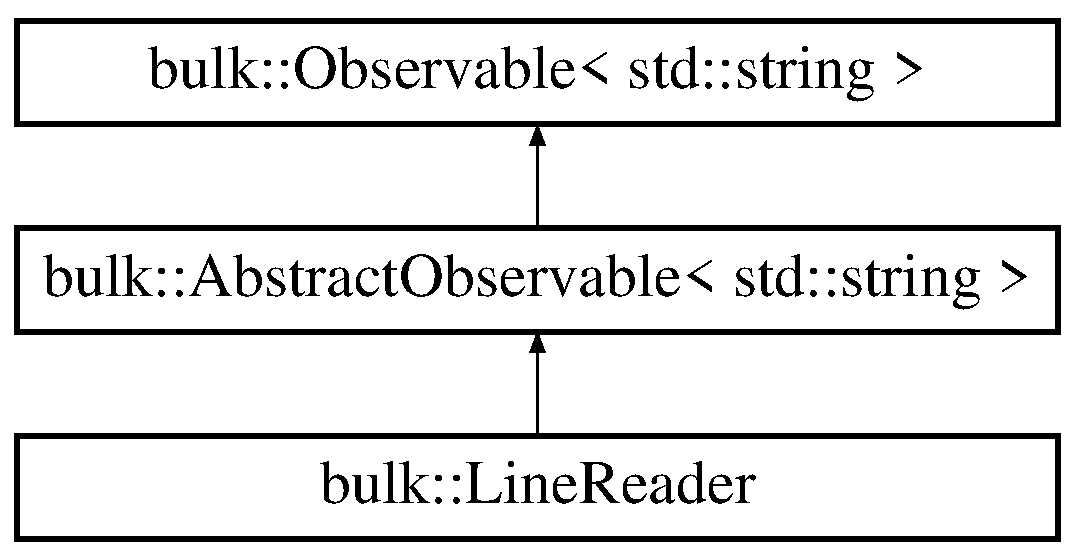
\includegraphics[height=3.000000cm]{classbulk_1_1LineReader}
\end{center}
\end{figure}
\subsection*{Public Member Functions}
\begin{DoxyCompactItemize}
\item 
\hyperlink{classbulk_1_1LineReader_aa257744aa82d916e0bbd16dd9766e88b}{$\sim$\+Line\+Reader} () override=default
\item 
\hyperlink{classbulk_1_1LineReader_aba7481f117f2155880d3e6b8e069633b}{Line\+Reader} (std\+::istream \&stream)
\item 
bool \hyperlink{classbulk_1_1LineReader_a8d0d6a11d162f9e020eed84e563a585f}{read\+\_\+line} ()
\end{DoxyCompactItemize}
\subsection*{Additional Inherited Members}


\subsection{Detailed Description}
Reads an input stream line-\/by-\/line, emits every line 

\subsection{Constructor \& Destructor Documentation}
\mbox{\Hypertarget{classbulk_1_1LineReader_aa257744aa82d916e0bbd16dd9766e88b}\label{classbulk_1_1LineReader_aa257744aa82d916e0bbd16dd9766e88b}} 
\index{bulk\+::\+Line\+Reader@{bulk\+::\+Line\+Reader}!````~Line\+Reader@{$\sim$\+Line\+Reader}}
\index{````~Line\+Reader@{$\sim$\+Line\+Reader}!bulk\+::\+Line\+Reader@{bulk\+::\+Line\+Reader}}
\subsubsection{\texorpdfstring{$\sim$\+Line\+Reader()}{~LineReader()}}
{\footnotesize\ttfamily bulk\+::\+Line\+Reader\+::$\sim$\+Line\+Reader (\begin{DoxyParamCaption}{ }\end{DoxyParamCaption})\hspace{0.3cm}{\ttfamily [override]}, {\ttfamily [default]}}

\mbox{\Hypertarget{classbulk_1_1LineReader_aba7481f117f2155880d3e6b8e069633b}\label{classbulk_1_1LineReader_aba7481f117f2155880d3e6b8e069633b}} 
\index{bulk\+::\+Line\+Reader@{bulk\+::\+Line\+Reader}!Line\+Reader@{Line\+Reader}}
\index{Line\+Reader@{Line\+Reader}!bulk\+::\+Line\+Reader@{bulk\+::\+Line\+Reader}}
\subsubsection{\texorpdfstring{Line\+Reader()}{LineReader()}}
{\footnotesize\ttfamily bulk\+::\+Line\+Reader\+::\+Line\+Reader (\begin{DoxyParamCaption}\item[{std\+::istream \&}]{stream }\end{DoxyParamCaption})\hspace{0.3cm}{\ttfamily [explicit]}}

Creates a reader, reading lines from the stream 
\begin{DoxyParams}{Parameters}
{\em stream} & Stream to read from \\
\hline
\end{DoxyParams}


\subsection{Member Function Documentation}
\mbox{\Hypertarget{classbulk_1_1LineReader_a8d0d6a11d162f9e020eed84e563a585f}\label{classbulk_1_1LineReader_a8d0d6a11d162f9e020eed84e563a585f}} 
\index{bulk\+::\+Line\+Reader@{bulk\+::\+Line\+Reader}!read\+\_\+line@{read\+\_\+line}}
\index{read\+\_\+line@{read\+\_\+line}!bulk\+::\+Line\+Reader@{bulk\+::\+Line\+Reader}}
\subsubsection{\texorpdfstring{read\+\_\+line()}{read\_line()}}
{\footnotesize\ttfamily bool bulk\+::\+Line\+Reader\+::read\+\_\+line (\begin{DoxyParamCaption}{ }\end{DoxyParamCaption})}

Attempts to read a single line \begin{DoxyReturn}{Returns}
true if reading was successful, false if E\+OF was reached, or other input error occurred 
\end{DoxyReturn}


The documentation for this class was generated from the following files\+:\begin{DoxyCompactItemize}
\item 
src/\hyperlink{line__reader_8hpp}{line\+\_\+reader.\+hpp}\item 
src/\hyperlink{line__reader_8cpp}{line\+\_\+reader.\+cpp}\end{DoxyCompactItemize}

\hypertarget{classbulk_1_1Observable}{}\section{bulk\+:\+:Observable$<$ T $>$ Class Template Reference}
\label{classbulk_1_1Observable}\index{bulk\+::\+Observable$<$ T $>$@{bulk\+::\+Observable$<$ T $>$}}


{\ttfamily \#include $<$observable.\+hpp$>$}

Inheritance diagram for bulk\+:\+:Observable$<$ T $>$\+:\begin{figure}[H]
\begin{center}
\leavevmode
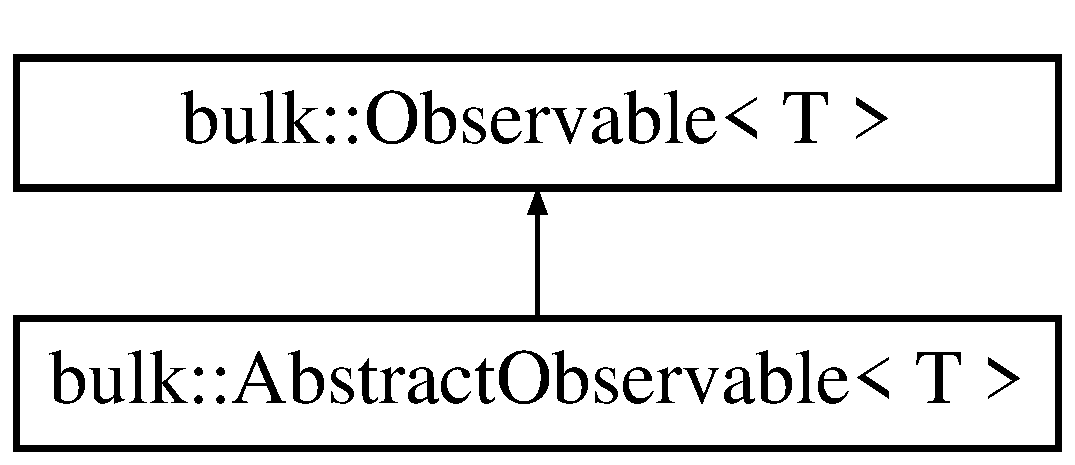
\includegraphics[height=2.000000cm]{classbulk_1_1Observable}
\end{center}
\end{figure}
\subsection*{Public Member Functions}
\begin{DoxyCompactItemize}
\item 
virtual \hyperlink{classbulk_1_1Observable_a4927059b909f8116927eb5275698153d}{$\sim$\+Observable} ()=default
\item 
virtual void \hyperlink{classbulk_1_1Observable_a1d014ef91398bff19bf96d9ef6bd5e10}{add\+\_\+subscriber} (const std\+::shared\+\_\+ptr$<$ \hyperlink{classbulk_1_1Observer}{Observer}$<$ T $>$$>$ \&observer)=0
\end{DoxyCompactItemize}


\subsection{Detailed Description}
\subsubsection*{template$<$typename T$>$\newline
class bulk\+::\+Observable$<$ T $>$}

Interface for observable of type T 
\begin{DoxyTemplParams}{Template Parameters}
{\em T} & Data type that is emitted by observable \\
\hline
\end{DoxyTemplParams}


\subsection{Constructor \& Destructor Documentation}
\mbox{\Hypertarget{classbulk_1_1Observable_a4927059b909f8116927eb5275698153d}\label{classbulk_1_1Observable_a4927059b909f8116927eb5275698153d}} 
\index{bulk\+::\+Observable@{bulk\+::\+Observable}!````~Observable@{$\sim$\+Observable}}
\index{````~Observable@{$\sim$\+Observable}!bulk\+::\+Observable@{bulk\+::\+Observable}}
\subsubsection{\texorpdfstring{$\sim$\+Observable()}{~Observable()}}
{\footnotesize\ttfamily template$<$typename T$>$ \\
virtual \hyperlink{classbulk_1_1Observable}{bulk\+::\+Observable}$<$ T $>$\+::$\sim$\hyperlink{classbulk_1_1Observable}{Observable} (\begin{DoxyParamCaption}{ }\end{DoxyParamCaption})\hspace{0.3cm}{\ttfamily [virtual]}, {\ttfamily [default]}}



\subsection{Member Function Documentation}
\mbox{\Hypertarget{classbulk_1_1Observable_a1d014ef91398bff19bf96d9ef6bd5e10}\label{classbulk_1_1Observable_a1d014ef91398bff19bf96d9ef6bd5e10}} 
\index{bulk\+::\+Observable@{bulk\+::\+Observable}!add\+\_\+subscriber@{add\+\_\+subscriber}}
\index{add\+\_\+subscriber@{add\+\_\+subscriber}!bulk\+::\+Observable@{bulk\+::\+Observable}}
\subsubsection{\texorpdfstring{add\+\_\+subscriber()}{add\_subscriber()}}
{\footnotesize\ttfamily template$<$typename T$>$ \\
virtual void \hyperlink{classbulk_1_1Observable}{bulk\+::\+Observable}$<$ T $>$\+::add\+\_\+subscriber (\begin{DoxyParamCaption}\item[{const std\+::shared\+\_\+ptr$<$ \hyperlink{classbulk_1_1Observer}{Observer}$<$ T $>$$>$ \&}]{observer }\end{DoxyParamCaption})\hspace{0.3cm}{\ttfamily [pure virtual]}}



Implemented in \hyperlink{classbulk_1_1AbstractObservable_a39be332eeed3b432a461faae184ba34b}{bulk\+::\+Abstract\+Observable$<$ T $>$}, \hyperlink{classbulk_1_1AbstractObservable_a39be332eeed3b432a461faae184ba34b}{bulk\+::\+Abstract\+Observable$<$ std\+::string $>$}, and \hyperlink{classbulk_1_1AbstractObservable_a39be332eeed3b432a461faae184ba34b}{bulk\+::\+Abstract\+Observable$<$ std\+::vector$<$ std\+::string $>$ $>$}.



The documentation for this class was generated from the following file\+:\begin{DoxyCompactItemize}
\item 
src/\hyperlink{observable_8hpp}{observable.\+hpp}\end{DoxyCompactItemize}

\hypertarget{classbulk_1_1Observer}{}\section{bulk\+:\+:Observer$<$ T $>$ Class Template Reference}
\label{classbulk_1_1Observer}\index{bulk\+::\+Observer$<$ T $>$@{bulk\+::\+Observer$<$ T $>$}}


{\ttfamily \#include $<$observable.\+hpp$>$}

\subsection*{Public Member Functions}
\begin{DoxyCompactItemize}
\item 
virtual \hyperlink{classbulk_1_1Observer_a64cb6e08300f80ab54b2417f45f57396}{$\sim$\+Observer} ()=default
\item 
virtual void \hyperlink{classbulk_1_1Observer_af17104660bf8b287e467213c4efbee2e}{update} (const T \&data)=0
\end{DoxyCompactItemize}


\subsection{Detailed Description}
\subsubsection*{template$<$typename T$>$\newline
class bulk\+::\+Observer$<$ T $>$}

Interface for observer of type T 
\begin{DoxyTemplParams}{Template Parameters}
{\em T} & Type of data the observer can process \\
\hline
\end{DoxyTemplParams}


\subsection{Constructor \& Destructor Documentation}
\mbox{\Hypertarget{classbulk_1_1Observer_a64cb6e08300f80ab54b2417f45f57396}\label{classbulk_1_1Observer_a64cb6e08300f80ab54b2417f45f57396}} 
\index{bulk\+::\+Observer@{bulk\+::\+Observer}!````~Observer@{$\sim$\+Observer}}
\index{````~Observer@{$\sim$\+Observer}!bulk\+::\+Observer@{bulk\+::\+Observer}}
\subsubsection{\texorpdfstring{$\sim$\+Observer()}{~Observer()}}
{\footnotesize\ttfamily template$<$typename T$>$ \\
virtual \hyperlink{classbulk_1_1Observer}{bulk\+::\+Observer}$<$ T $>$\+::$\sim$\hyperlink{classbulk_1_1Observer}{Observer} (\begin{DoxyParamCaption}{ }\end{DoxyParamCaption})\hspace{0.3cm}{\ttfamily [virtual]}, {\ttfamily [default]}}



\subsection{Member Function Documentation}
\mbox{\Hypertarget{classbulk_1_1Observer_af17104660bf8b287e467213c4efbee2e}\label{classbulk_1_1Observer_af17104660bf8b287e467213c4efbee2e}} 
\index{bulk\+::\+Observer@{bulk\+::\+Observer}!update@{update}}
\index{update@{update}!bulk\+::\+Observer@{bulk\+::\+Observer}}
\subsubsection{\texorpdfstring{update()}{update()}}
{\footnotesize\ttfamily template$<$typename T$>$ \\
virtual void \hyperlink{classbulk_1_1Observer}{bulk\+::\+Observer}$<$ T $>$\+::update (\begin{DoxyParamCaption}\item[{const T \&}]{data }\end{DoxyParamCaption})\hspace{0.3cm}{\ttfamily [pure virtual]}}



Implemented in \hyperlink{classbulk_1_1BlockReader_a0a3b9ff69552b233b037afcd7e858ef1}{bulk\+::\+Block\+Reader}, and \hyperlink{classbulk_1_1BlockPrinter_a9f961b39d2c0bf9112524bf6773bb3e1}{bulk\+::\+Block\+Printer}.



The documentation for this class was generated from the following file\+:\begin{DoxyCompactItemize}
\item 
src/\hyperlink{observable_8hpp}{observable.\+hpp}\end{DoxyCompactItemize}

\chapter{File Documentation}
\hypertarget{block__file__printer_8cpp}{}\section{src/block\+\_\+file\+\_\+printer.cpp File Reference}
\label{block__file__printer_8cpp}\index{src/block\+\_\+file\+\_\+printer.\+cpp@{src/block\+\_\+file\+\_\+printer.\+cpp}}
{\ttfamily \#include \char`\"{}block\+\_\+file\+\_\+printer.\+hpp\char`\"{}}\newline
{\ttfamily \#include $<$chrono$>$}\newline
{\ttfamily \#include $<$fstream$>$}\newline

\hypertarget{block__file__printer_8hpp}{}\section{src/block\+\_\+file\+\_\+printer.hpp File Reference}
\label{block__file__printer_8hpp}\index{src/block\+\_\+file\+\_\+printer.\+hpp@{src/block\+\_\+file\+\_\+printer.\+hpp}}
{\ttfamily \#include \char`\"{}observable.\+hpp\char`\"{}}\newline
{\ttfamily \#include $<$vector$>$}\newline
{\ttfamily \#include $<$string$>$}\newline
\subsection*{Classes}
\begin{DoxyCompactItemize}
\item 
class \hyperlink{classbulk_1_1BlockFilePrinter}{bulk\+::\+Block\+File\+Printer}
\begin{DoxyCompactList}\small\item\em Saves each block into a separate file file name format\+: bulk123456.\+log Where 123456 is the timestamp in seconds. \end{DoxyCompactList}\end{DoxyCompactItemize}
\subsection*{Namespaces}
\begin{DoxyCompactItemize}
\item 
 \hyperlink{namespacebulk}{bulk}
\end{DoxyCompactItemize}

\hypertarget{block__printer_8cpp}{}\section{src/block\+\_\+printer.cpp File Reference}
\label{block__printer_8cpp}\index{src/block\+\_\+printer.\+cpp@{src/block\+\_\+printer.\+cpp}}
{\ttfamily \#include \char`\"{}block\+\_\+printer.\+hpp\char`\"{}}\newline

\hypertarget{block__printer_8hpp}{}\section{src/block\+\_\+printer.hpp File Reference}
\label{block__printer_8hpp}\index{src/block\+\_\+printer.\+hpp@{src/block\+\_\+printer.\+hpp}}
{\ttfamily \#include \char`\"{}observable.\+hpp\char`\"{}}\newline
{\ttfamily \#include $<$memory$>$}\newline
{\ttfamily \#include $<$ostream$>$}\newline
{\ttfamily \#include $<$vector$>$}\newline
{\ttfamily \#include $<$string$>$}\newline
\subsection*{Classes}
\begin{DoxyCompactItemize}
\item 
class \hyperlink{classbulk_1_1BlockPrinter}{bulk\+::\+Block\+Printer}
\end{DoxyCompactItemize}
\subsection*{Namespaces}
\begin{DoxyCompactItemize}
\item 
 \hyperlink{namespacebulk}{bulk}
\end{DoxyCompactItemize}

\hypertarget{block__reader_8cpp}{}\section{src/block\+\_\+reader.cpp File Reference}
\label{block__reader_8cpp}\index{src/block\+\_\+reader.\+cpp@{src/block\+\_\+reader.\+cpp}}
{\ttfamily \#include \char`\"{}block\+\_\+reader.\+hpp\char`\"{}}\newline

\hypertarget{block__reader_8hpp}{}\section{src/block\+\_\+reader.hpp File Reference}
\label{block__reader_8hpp}\index{src/block\+\_\+reader.\+hpp@{src/block\+\_\+reader.\+hpp}}
{\ttfamily \#include \char`\"{}observable.\+hpp\char`\"{}}\newline
{\ttfamily \#include $<$cstddef$>$}\newline
{\ttfamily \#include $<$memory$>$}\newline
{\ttfamily \#include $<$vector$>$}\newline
{\ttfamily \#include $<$string$>$}\newline
\subsection*{Classes}
\begin{DoxyCompactItemize}
\item 
class \hyperlink{classbulk_1_1BlockReader}{bulk\+::\+Block\+Reader}
\end{DoxyCompactItemize}
\subsection*{Namespaces}
\begin{DoxyCompactItemize}
\item 
 \hyperlink{namespacebulk}{bulk}
\end{DoxyCompactItemize}

\hypertarget{CMakeLists_8txt}{}\section{src/\+C\+Make\+Lists.txt File Reference}
\label{CMakeLists_8txt}\index{src/\+C\+Make\+Lists.\+txt@{src/\+C\+Make\+Lists.\+txt}}

\hypertarget{line__reader_8cpp}{}\section{src/line\+\_\+reader.cpp File Reference}
\label{line__reader_8cpp}\index{src/line\+\_\+reader.\+cpp@{src/line\+\_\+reader.\+cpp}}
{\ttfamily \#include \char`\"{}line\+\_\+reader.\+hpp\char`\"{}}\newline

\hypertarget{line__reader_8hpp}{}\section{src/line\+\_\+reader.hpp File Reference}
\label{line__reader_8hpp}\index{src/line\+\_\+reader.\+hpp@{src/line\+\_\+reader.\+hpp}}


Header file for Line\+Reader class.  


{\ttfamily \#include \char`\"{}observable.\+hpp\char`\"{}}\newline
{\ttfamily \#include $<$istream$>$}\newline
\subsection*{Classes}
\begin{DoxyCompactItemize}
\item 
class \hyperlink{classbulk_1_1LineReader}{bulk\+::\+Line\+Reader}
\end{DoxyCompactItemize}
\subsection*{Namespaces}
\begin{DoxyCompactItemize}
\item 
 \hyperlink{namespacebulk}{bulk}
\end{DoxyCompactItemize}


\subsection{Detailed Description}
Header file for Line\+Reader class. 

\begin{DoxyAuthor}{Author}
ktori 
\end{DoxyAuthor}

\hypertarget{main_8cpp}{}\section{src/main.cpp File Reference}
\label{main_8cpp}\index{src/main.\+cpp@{src/main.\+cpp}}
\subsection*{Functions}
\begin{DoxyCompactItemize}
\item 
int \hyperlink{main_8cpp_ae66f6b31b5ad750f1fe042a706a4e3d4}{main} ()
\end{DoxyCompactItemize}


\subsection{Function Documentation}
\mbox{\Hypertarget{main_8cpp_ae66f6b31b5ad750f1fe042a706a4e3d4}\label{main_8cpp_ae66f6b31b5ad750f1fe042a706a4e3d4}} 
\index{main.\+cpp@{main.\+cpp}!main@{main}}
\index{main@{main}!main.\+cpp@{main.\+cpp}}
\subsubsection{\texorpdfstring{main()}{main()}}
{\footnotesize\ttfamily int main (\begin{DoxyParamCaption}{ }\end{DoxyParamCaption})}


\hypertarget{observable_8hpp}{}\section{src/observable.hpp File Reference}
\label{observable_8hpp}\index{src/observable.\+hpp@{src/observable.\+hpp}}
{\ttfamily \#include $<$memory$>$}\newline
{\ttfamily \#include $<$forward\+\_\+list$>$}\newline
\subsection*{Classes}
\begin{DoxyCompactItemize}
\item 
class \hyperlink{classbulk_1_1Observer}{bulk\+::\+Observer$<$ T $>$}
\item 
class \hyperlink{classbulk_1_1Observable}{bulk\+::\+Observable$<$ T $>$}
\item 
class \hyperlink{classbulk_1_1AbstractObservable}{bulk\+::\+Abstract\+Observable$<$ T $>$}
\end{DoxyCompactItemize}
\subsection*{Namespaces}
\begin{DoxyCompactItemize}
\item 
 \hyperlink{namespacebulk}{bulk}
\end{DoxyCompactItemize}

%--- End generated contents ---

% Index
\backmatter
\newpage
\phantomsection
\clearemptydoublepage
\addcontentsline{toc}{chapter}{Index}
\printindex

\end{document}
